\documentclass{standalone}

%----------------------------------------------------------------------------------------------%
%                                 Packages and basic declarations
%----------------------------------------------------------------------------------------------%

\usepackage[utf8]{inputenc}
\usepackage{pgfplots}
\usepackage{tikz}
\usepackage{nicefrac}


%----------------------------------------------------------------------------------------------%
%----------------------------------------------------------------------------------------------%
%                                            DOCUMENT STARTS
%----------------------------------------------------------------------------------------------%
%----------------------------------------------------------------------------------------------%


\begin{document}

\def\markersize{4.5pt}
\def\linewidth{3.pt}

%Tikz picture starts%

\begin{tikzpicture}

%Tikz axis starts%

\begin{axis}[width=30cm,
% SCALE
scale=0.5,
% STYLE
%title style={font=\fontsize{40}{8}\selectfont},
xlabel style={at={(axis description cs:0.5,-0.025)},anchor=north,font=\fontsize{48}{40}\selectfont},
ylabel style={at={(axis description cs:-0.05,.5)},anchor=south,font=\fontsize{48}{40}\selectfont},
tick align=outside,
tick label style={font=\huge},
legend style={draw=white!80.0!black,font=\fontsize{19}{14}\selectfont,row sep=8pt},
legend image post style={xscale=1.25,yscale=1.25},
legend cell align={left},
clip mode=individual,
% GRID STYLE
xmajorgrids,
x grid style={lightgray!92.026143790849673!black},
ymajorgrids,
y grid style={lightgray!92.026143790849673!black},
line width=0.75mm,
% GRID SIZE
%xmin=0.0,
xmax=75.0,
ymin=0.0,
%xtick={0.0,10.0,30.0,50.0,70.0,90.0,110.0,130.0,150.0},
% CONTENT
%title={\bf{$\frac{G_{I}}{G_{0}}$ as function of debond's size $\Delta\theta$, in-house VCCT routine}},
xlabel={$\Delta\theta\left[^{\circ}\right]$},
ylabel={$G\left[\nicefrac{J}{m^{2}}\right]$},
% LEGEND ENTRIES
%legend entries={{$3\times 2-free$},{$5\times 2-free$},{$5\times 3-free$},{$11\times 2-free$},{$11\times 6-free$},{$21\times 2-free$},{$21\times 11-free$},{$101\times 2-free$},{$101\times 11-free$},{$201\times 2-free$},{$201\times 11-free$}},
legend pos={south east},
legend entries={},
]
%$21\times 21-free$

%% SF1, AF1
%\addplot[line width=\linewidth,mark size=\markersize,black,smooth,mark=square*]
%table{
%10.00	0.68801176
%20.00	1.34581140
%30.00	2.00966243
%40.00	2.48063159
%50.00	2.79238090
%60.00	2.93023840
%70.00	2.71211738
%80.00	2.28624094
%90.00	1.80318221
%100.00	1.16861842
%110.00	0.57815971
%120.00	0.23781140
%130.00	0.09368958
%140.00	0.03445403
%150.00	0.01253746
%};

%% SF2, AF1
%\addplot[line width=\linewidth,mark size=\markersize,red,smooth,mark=square*]
%table{
%10.00	0.71911006
%20.00	1.51842309
%30.00	2.44491584
%40.00	3.18358399
%50.00	3.68020891
%60.00	3.90198008
%70.00	3.65465733
%80.00	3.18696867
%90.00	2.58864650
%100.00	1.71185365
%110.00	0.86236181
%120.00	0.35943790
%130.00	0.13533614
%140.00	0.03951343
%150.00	0.00621640
%};
%
%% SF2, AF2
%\addplot[line width=\linewidth,mark size=\markersize,red!70!black,smooth,mark=triangle*]
%table{
%10.00	0.71666394
%20.00	1.50007363
%30.00	2.39628382
%40.00	3.10852234
%50.00	3.58792238
%60.00	3.80589293
%70.00	3.58043772
%80.00	3.10079302
%90.00	2.53226142
%100.00	1.72055000
%110.00	0.90779311
%120.00	0.40130416
%130.00	0.16186128
%140.00	0.05250992
%150.00	0.01054751
%};
%
%% SF5, AF1
%\addplot[line width=\linewidth,mark size=\markersize,green,smooth,mark=square*]
%table{
%10.00	0.73351529
%20.00	1.60313771
%30.00	2.67327334
%40.00	3.59768155
%50.00	4.27691025
%60.00	4.64474155
%70.00	4.44920337
%80.00	3.97146152
%90.00	3.29239637
%100.00	2.21154655
%110.00	1.12632728
%120.00	0.47267367
%130.00	0.17747036
%140.00	0.05021628
%150.00	0.00674539
%};
%
%% SF5, AF5
%\addplot[line width=\linewidth,mark size=\markersize,green!70!black,smooth,mark=triangle*]
%table{
%10.00	0.72822190
%20.00	1.57183944
%30.00	2.58991862
%40.00	3.45252402
%50.00	4.06822315
%60.00	4.38414928
%70.00	4.18782003
%80.00	3.68312642
%90.00	3.05887247
%100.00	2.12281092
%110.00	1.14830875
%120.00	0.51990353
%130.00	0.21204532
%140.00	0.06722982
%150.00	0.01157588
%};

\node [above right] at (rel axis cs:0.015,0.575) {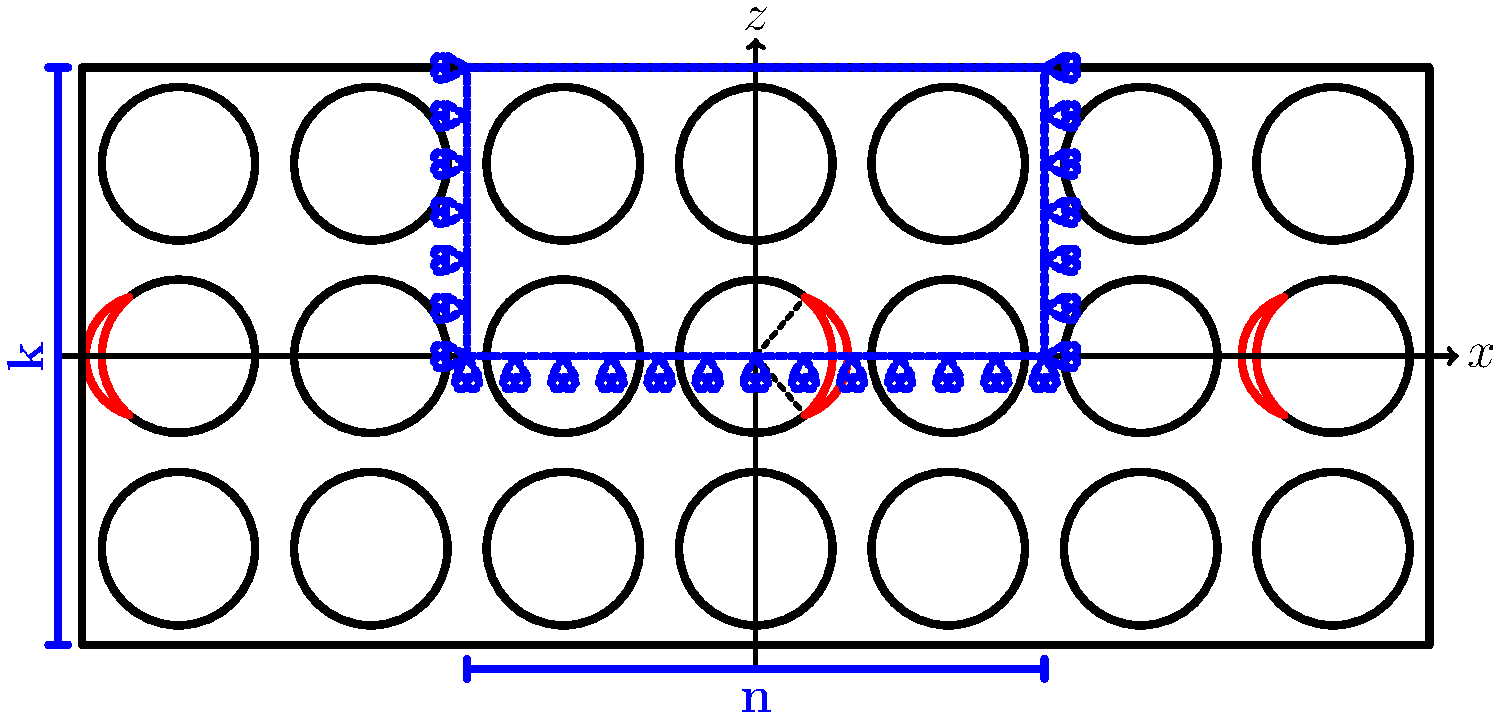
\includegraphics[width=10cm]{thickPly.pdf}};

\node [right] at (rel axis cs:0.2,0.545) {\LARGE$\mathbf{21\times 21-free}$};

\draw[line width=0.5mm] (rel axis cs:0.375,0.515) -- (rel axis cs:0.275,0.365) ;

% SF10, AF10
\addplot[line width=\linewidth,mark size=\markersize,red,smooth,mark=square*]
table[x=theta, y expr={\thisrow{GI} + \thisrow{GII}}]{
theta    GI                 GII
10.00	  3.53079692 0.72745157
20.00	  3.57968267 1.58361364
30.00	  2.85235663 2.62415975
40.00	  1.89413525 3.51755089
50.00	  1.00169026 4.16619181
60.00	  0.29150430 4.51054060
70.00	  0.00035418 4.32694752
80.00   0.00006936 3.81995778
90.00	  0.00007606 3.18341270
100.00 0.00007286 2.21668480
110.00 0.00003954 1.20227684
120.00 0.00001867 0.54528508
130.00 0.00000644 0.22249952
140.00 0.00000112 0.07042414
150.00 0.00201653 0.01200957
};
\addlegendentry{$G_{TOT}$}

\def\GIref{3.53079692 }
\def\GIIref{0.72745157}
\def\lambda{0.35}
\pgfmathsetmacro\GTOTref{\GIref+\GIIref}
\pgfmathsetmacro\psiref{rad(atan(sqrt(\GIIref/\GIref)))}
\pgfmathsetmacro\ratioref{1+(tan(deg((1-\lambda)*\psiref)))^(2)}
\pgfmathsetmacro\GIc{\GTOTref/\ratioref}


% SF10, AF10
\addplot[line width=\linewidth,mark size=\markersize,blue,smooth,mark=*,mark options={fill=white}]
table[x=theta, y expr={\GIc*(1+(tan(deg((1-\lambda)*rad(atan(sqrt(\thisrow{GII}/\thisrow{GI}))))))^(2))}]{
theta    GI                 GII
10.00	  3.53079692 0.72745157
20.00	  3.57968267 1.58361364
30.00	  2.85235663 2.62415975
40.00	  1.89413525 3.51755089
50.00	  1.00169026 4.16619181
60.00	  0.29150430 4.51054060
70.00	  0.00035418 4.32694752
80.00   0.00006936 3.81995778
90.00	  0.00007606 3.18341270
100.00 0.00007286 2.21668480
110.00 0.00003954 1.20227684
120.00 0.00001867 0.54528508
130.00 0.00000644 0.22249952
140.00 0.00000112 0.07042414
150.00 0.00201653 0.01200957
};
\addlegendentry{$G_{c}, \Delta\theta_{ref}=10^{\circ}$}

\def\lambda{0.35}

\def\GIten{3.53079692}
\def\GIIten{0.72745157}
\def\GItwe{3.57968267}
\def\GIItwe{1.58361364}

\pgfmathsetmacro\mI{(\GItwe-\GIten)/(10.0)}

\pgfmathsetmacro\GIref{\GIten+\mI*(-10.0)}
\pgfmathsetmacro\GIIref{0.0}

\pgfmathsetmacro\GTOTref{\GIref+\GIIref}
\pgfmathsetmacro\psiref{rad(atan(sqrt(\GIIref/\GIref)))}
\pgfmathsetmacro\ratioref{1+(tan(deg((1-\lambda)*\psiref)))^(2)}
\pgfmathsetmacro\GIc{\GTOTref/\ratioref}


% SF10, AF10
\addplot[line width=\linewidth,mark size=\markersize,green,smooth,mark=diamond*,mark options={fill=white}]
table[x=theta, y expr={\GIc*(1+(tan(deg((1-\lambda)*rad(atan(sqrt(\thisrow{GII}/\thisrow{GI}))))))^(2))}]{
theta    GI                 GII
10.00	  3.53079692 0.72745157
20.00	  3.57968267 1.58361364
30.00	  2.85235663 2.62415975
40.00	  1.89413525 3.51755089
50.00	  1.00169026 4.16619181
60.00	  0.29150430 4.51054060
70.00	  0.00035418 4.32694752
80.00   0.00006936 3.81995778
90.00	  0.00007606 3.18341270
100.00 0.00007286 2.21668480
110.00 0.00003954 1.20227684
120.00 0.00001867 0.54528508
130.00 0.00000644 0.22249952
140.00 0.00000112 0.07042414
150.00 0.00201653 0.01200957
};
\addlegendentry{$G_{c}, \Delta\theta_{ref}=0^{\circ}$}

%% SF50, AF1
%\addplot[line width=\linewidth,mark size=\markersize,magenta,smooth,mark=square*]
%table{
%10.00	0.73877781
%20.00	1.65566200
%30.00	2.82335394
%40.00	3.89196505
%50.00	4.73594005
%60.00	5.25955675
%70.00	5.14410521
%80.00	4.67949013
%90.00	3.94439342
%100.00	2.68341057
%110.00	1.37702310
%120.00	0.57991961
%130.00	0.21802903
%140.00	0.06171126
%150.00	0.00828550
%};
%
%% SF50, AF5
%\addplot[line width=\linewidth,mark size=\markersize,magenta!70!black,smooth,mark=triangle*]
%table{
%10.00	0.73194862
%20.00	1.59196088
%30.00	2.64702514
%40.00	3.55981162
%50.00	4.22897192
%60.00	4.59164750
%70.00	4.41606521
%80.00	3.91294040
%90.00	3.26841547
%100.00	2.27356614
%110.00	1.22825358
%120.00	0.55388902
%130.00	0.22430908
%140.00	0.07000755
%150.00	0.01141913
%};
%
%% SF100, AF1
%\addplot[line width=\linewidth,mark size=\markersize,gray,smooth,mark=square*]
%table{
%10.00	0.74278107
%20.00	1.65813914
%30.00	2.83284204
%40.00	3.91081824
%50.00	4.76610494
%60.00	5.30070491
%70.00	5.19142775
%80.00	4.72842097
%90.00	3.99008365
%100.00	2.71672455
%110.00	1.39480854
%120.00	0.58754808
%130.00	0.22092971
%140.00	0.06254366
%150.00	0.00840009
%};
%
%% SF100, AF5
%\addplot[line width=\linewidth,mark size=\markersize,gray!70!black,smooth,mark=triangle*]
%table{
%10.00	0.73178460
%20.00	1.59344231
%30.00	2.64884474
%40.00	3.56382249
%50.00	4.23562842
%60.00	4.60052034
%70.00	4.42606610
%80.00	3.92307977
%90.00	3.27733981
%100.00	2.28034136
%110.00	1.23205780
%120.00	0.55563612
%130.00	0.22502102
%140.00	0.07022368
%150.00	0.01145254
%};
\end{axis}
%Tikz axis ends%


\end{tikzpicture}
%Tikz picture ends%


\end{document}

%----------------------------------------------------------------------------------------------%
%----------------------------------------------------------------------------------------------%
%                                            DOCUMENT ENDS
%----------------------------------------------------------------------------------------------%
%----------------------------------------------------------------------------------------------%
